\chapter{Background}
%The background should set the project into context by motivating the subject matter and relating it to existing published work. The background will include a critical evaluation of the existing literature in the area in which your project work is based and should lead the reader to understand how your work is motivated by and related to existing work.

For my BSc individual project, I will be researching procedural content generation (PCG) algorithms and then implementing them each in a small 3D game made with the Godot Engine (and its domain-specific GDScript language).

\section{Procedural Generation: Background}

\href{https://en.wikipedia.org/wiki/Procedural_generation}{Procedural content generation} (usually referred to as simply ``procedural generation") refers to the creation of levels and other game objects programmatically and algorithmically, in lieu of a human being doing all the work. While procedural generation algorithms can be used to generate a myriad of things, from textures (for things like trees and clouds) to music (``generative music," as coined by legendary musician Brian Eno), by far its most common context is in automated level design, generating level layouts algorithmically in lieu of work from level designers. Game developers may opt to use procedural generation to save time and money designing levels or show off technical prowess in their games.

\href{https://en.wikipedia.org/wiki/Procedural\_generation#Video\_games}{Procedural generation in video games has a rich history.} Pioneering games such as Rogue (1980) took direct influence from tabletop role-playing games such as Dungeons and Dragons, and thus had a player navigate a randomly-generated world that expanded further as they went on. Such games spawned the \emph{roguelike} and \emph{roguelite} genres, which experienced immense popularity in the last decade. In the realm of first-person shooters, 2004's .kkrieger, as seen in Figure \ref{fig:kkrieger}, used procedural generation to create intricate 3D levels and fit them all into a game that takes up just 96 kilobytes of space. 

%\begin{figure}[H]
%	\centering
%	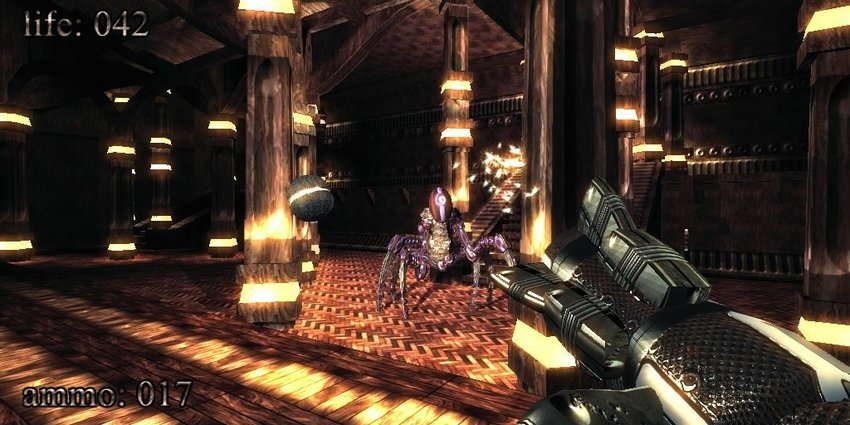
\includegraphics[width=0.75\textwidth]{kkrieger.png}
%	\caption{The game .kkrieger, which uses procedural generation to design maps while keeping the game at a 96 kilobyte file size.\\Source: \link{https://www.researchgate.net/figure/The-game-kkrieger-has-a-file-size-of-96-kb\_fig1\_320722498}}
%	\label{fig:kkrieger}
%\end{figure}

Other games that use procedural generation in its levels include Elite (originally published in 1984), Elite: Dangerous (2012), Minecraft (2009), No Man's Sky (2012) and Spelunky (2013). \href{https://youtu.be/Uqk5Zf0tw3o}{The latter game's use of procedural generation has notably been covered by video games journalist Mark Brown in a YouTube video.}

%\begin{figure}[H]
%	\centering
%	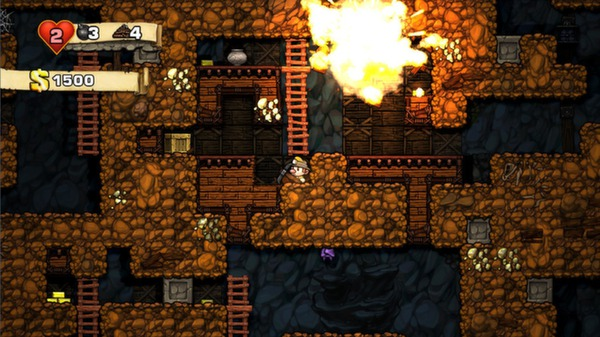
\includegraphics[width=0.7\textwidth]{spelunky.jpg}
%	\caption{\href{https://spelunkyworld.com/}{The roguelike game Spelunky}, which uses procedural generation to build intricate levels for the player character to explore.\\Source: \link{https://store.steampowered.com/app/239350/Spelunky/}}
%	\label{fig:spelunky}
%\end{figure}

In many cases, these games end up having a \textbf{large} number of different environments that each game could generate for its players. However, by procedurally generating them upon the \textit{loading} of the game level, in lieu of loading a layout from disk, they can save a lot of space (albeit with a considerable need for processing power, depending on the game's and algorithms' performance), as seen with .kkrieger.% in Figure \ref{fig:kkrieger}.

Using one or some different procedural generation algorithms, such as the use of Perlin, Simplex or other noise, Voronoï disks and also poisson disk generation, among others, games can load a seed to randomly generate a level every time it is played, meaning no two playthroughs of a game with procedurally generated content are ever the same.

\section{Justifying My Choice of Engine: Godot}

While a myriad of resources exist for procedurally generated game contents exist for Unity and Unreal, I want to implement them in Godot, for several reasons:

\begin{itemize}
	\item It's the engine I have the most experience with, having already developed 2 published web games with it.
	\item It's not got as many resources on procedural generation compared to Unity, Unreal and some other popular game engines, particularly on the side of academic research (that is, there aren't as many papers on procedural generation that pertain to Godot as they do to Unity, Unreal and other engines).
	\begin{itemize}
		\item However, it is still very powerful and feature-rich (it has its own Open Simplex noise class, for example) and I'm sure I can make procedural generation algorithms work on it.
	\end{itemize}
	\item Compared to Unity and Unreal, Godot is a very light engine with a feature-rich editor, clocking in at under 100MB, with editors for Windows, macOS, Linux and even the web browser. 
\end{itemize}

By the end of my allotted time, I plan to have implemented several procedurally generated environments in small Godot games, using a myriad of methods (such as Voronoï cell and poisson disk generation) in a myriad of contexts (anything from platformers to first-person games). With these games, I plan for the final report to be the centrepiece of my project, with it containing my research on how each environment was implemented, as well as my findings on the algorithms themselves and how they work.

This is more a research-oriented project than an implementation-oriented project, but the implementations will nonetheless prove that Godot is just as adept at procedural content generation as the other major players in the game engine space, and I will have gained immense knowledge on PCG in the process. 